%==============================================================================
%  MATH 231 -- Linear Algebra I (Queens College, Fall 2026)
%  MATRIX UNIT, PART 6 -- The Null Space and Rank-Nullity
%
%  Section numbering runs CONTINUOUSLY across the parts of the matrix unit;
%  see Part 2's header for the full map.  This part is Sections 30-34, hence
%  \setcounter{section}{29}.
%
%  STATUS: complete.  Sections 30-34.  Written from the plan in
%  plan/MATH231_remaining_units_plan.tex (2026-10-25).
%
%  AUDIENCE: distributed to students.  No instructor-facing apparatus.
%
%  WHAT THE INSTRUCTOR SPECIFIED, AND WHERE IT IS.
%   - Returning to column and row space: full rank, rank deficiency, mapping
%     vectors from one space into the other, subspaces, a matrix-invariant
%     subspace: Sec. 30.
%   - Null space, kernel, nullity, simple examples: Sec. 31.
%   - The relationship between rank and null space; the rank-nullity theorem
%     with a straightforward proof and many simple examples: Sec. 32.
%   - The corollary rank(A) = rank(A'A) with a straightforward proof from
%     rank-nullity: Sec. 33.1-33.2.
%   - The 2x2 inverse: Sec. 34.
%
%  DECISIONS CARRIED FROM THE PLAN.
%
%   D4. ROW RANK = COLUMN RANK is proved in Sec. 33.3 as a second corollary
%       of rank(A'A) = rank(A): col[A'A] is inside col[A'], so rank A <=
%       rank A'; apply it to A' for the reverse.  This settles the promise
%       made in Sec. 12.4 without elimination.
%
%   D5. RANK-NULLITY BEFORE ELIMINATION.  The proof in Sec. 32.3 extends a
%       basis of the null space to a basis of R^n.  It takes as given three
%       facts about dimension (F1-F3, stated in Sec. 32.3) that the course
%       has used but never proved in general -- the same footing on which
%       Part 1 Sec. 1.1 accepted "n independent vectors span R^n".  Sec. 43.4
%       gives the second, computational proof by counting pivots.
%
%   NOTATION (plan N1).  null[A] for the null space, in the style of col[A]
%   and row[A]; kernel, N(A) and ker A are mentioned once.  Subspaces take
%   brackets, numbers take parentheses: rank(A), nullity(A).
%
%   2x2 INVERSE (Sec. 34) is derived by solving AX = I column by column, as
%   in the plan.  The general inverse is Part 10.
%
%   INVARIANT SUBSPACES (Sec. 30.4) end with a pointer to eigenvectors; it
%   is phrased as "the next unit" so it survives any renumbering.
%
%  Compile with pdflatex or tectonic (standard TeX Live packages only; uses
%  tikz).
%==============================================================================
\documentclass[11pt]{article}

\usepackage[margin=1in]{geometry}
\usepackage{amsmath,amssymb,amsthm}
\usepackage[dvipsnames]{xcolor}
\usepackage{enumitem}
\usepackage{booktabs}
\usepackage{array}
\usepackage[hidelinks]{hyperref}
\usepackage{titlesec}
\usepackage{needspace}
\usepackage{tikz}
\usetikzlibrary{arrows.meta}

%------------------------------------------------------------------ style ----
\titleformat{\section}{\large\bfseries\sffamily}{\thesection.}{0.6em}{}
\titleformat{\subsection}{\normalsize\bfseries\sffamily}{\thesubsection.}{0.5em}{}
\titlespacing*{\section}{0pt}{14pt}{6pt}
\setlength{\emergencystretch}{3em}

\theoremstyle{plain}
\newtheorem{thm}{Theorem}[section]
\newtheorem{lem}[thm]{Lemma}
\newtheorem{cor}[thm]{Corollary}

\theoremstyle{definition}
\newtheorem{defn}{Definition}[section]
\newtheorem{ex}{Example}[section]
\theoremstyle{remark}
\newtheorem*{rmk}{Remark}
\newtheorem*{warn}{A common confusion}

\newcommand{\lookahead}{\par\smallskip\noindent
  \textbf{\sffamily\textcolor{RoyalBlue}{Looking ahead.}}\ \ignorespaces}
\newcommand{\lookback}[1][the vector unit]{\par\smallskip\noindent
  \textbf{\sffamily\textcolor{ForestGreen}{From #1.}}\ \ignorespaces}

%--------------------------------------------------------------- notation ----
\newcommand{\R}{\mathbb{R}}
\newcommand{\vc}[1]{\mathbf{#1}}
\newcommand{\mt}[1]{\mathbf{#1}}
\newcommand{\norm}[1]{\lVert #1\rVert}
\newcommand{\T}{^{\mathsf{T}}}
\newcommand{\smat}[1]{\left[\begin{smallmatrix}#1\end{smallmatrix}\right]}
\newcommand{\colsp}[1]{\operatorname{col}[#1]}
\newcommand{\rowsp}[1]{\operatorname{row}[#1]}
\newcommand{\nullsp}[1]{\operatorname{null}[#1]}
\DeclareMathOperator{\spanop}{span}
\DeclareMathOperator{\diagop}{diag}
\DeclareMathOperator{\rank}{rank}
\DeclareMathOperator{\nullity}{nullity}

%------------------------------------------------------------- tikz helpers --
\tikzset{
  vecarr/.style   = {-{Stealth[length=2.6mm,width=2.0mm]},very thick},
  thinarr/.style  = {-{Stealth[length=2.2mm,width=1.7mm]},thick},
  axisline/.style = {->,gray!75,thin}
}

\title{\vspace{-1.2cm}\textbf{\sffamily MATH 231 -- Linear Algebra I}\\[4pt]
       {\large\sffamily The Matrix Unit, Part 6 \textbullet\ The Null Space
        and Rank--Nullity}\\[2pt]
       {\normalsize\sffamily Kiely Hall 326 \textbullet\
        Instructor: Kevin Bedoya}}
\author{}
\date{}

\begin{document}
\setcounter{section}{29}  % this part opens at Section 30; see the header note
\maketitle
\vspace{-1.6cm}

\noindent\textbf{About this document.} This is Part 6 of the matrix unit,
Sections 30--34. Section numbers run continuously through the unit (Part 2's
opening table lists them all). References into the vector unit always name it.

\medskip
\noindent\textbf{Assumed.} The column space, row space and rank (\S10--\S12);
a matrix as a linear transformation (\S13); the $2\times2$ determinant and its
link to rank (\S14, \S22); projections and invariant lines met in Part 5. From
the vector unit: linear independence, basis and dimension (\S16--\S18, \S24),
and subspaces (\S19).

\medskip
\noindent\textbf{What you should be able to do afterwards.} Say whether a
matrix has full rank, full column rank, or full row rank; recognise invariant
subspaces of simple matrices; find the null space of a small matrix and its
nullity; describe the full solution set of $\mt{A}\vc{x}=\vc{b}$ as one solution
plus the null space; state and prove the rank--nullity theorem and use it to
predict nullities; prove that $\rank(\mt{A}\T\mt{A})=\rank(\mt{A})$ and that row
rank equals column rank; and invert a $2\times2$ matrix, or say why it cannot be
inverted.

%==============================================================================
\section{Column and row space, revisited}
%==============================================================================

%------------------------------------------------------------------------------
\subsection{Full rank and rank deficiency}
%------------------------------------------------------------------------------
\S12.2 showed that $\rank(\mt{A})\le\min(m,n)$ for $\mt{A}\in\R^{m\times n}$.
Reaching that bound is the best a matrix can do, and it has a name.

\begin{defn}[Full rank]
$\mt{A}\in\R^{m\times n}$ has \textbf{full rank} if $\rank(\mt{A})=\min(m,n)$,
and is \textbf{rank-deficient} otherwise. More specifically, $\mt{A}$ has
\textbf{full column rank} if $\rank(\mt{A})=n$ (its columns are independent),
and \textbf{full row rank} if $\rank(\mt{A})=m$ (its rows are independent, or
equivalently $\colsp{\mt{A}}=\R^{m}$).
\end{defn}

\noindent For a tall matrix ($m>n$), full rank means full column rank. For a
wide one ($m<n$), it means full row rank. For a square one, it means both.

\begin{ex}
\leavevmode
\begin{itemize}[leftmargin=1.4em,itemsep=2pt]
  \item $\begin{bmatrix}1&2\\3&4\end{bmatrix}$: rank $2$, full rank.
  \item $\begin{bmatrix}1&2\\2&4\end{bmatrix}$: rank $1<2$, rank-deficient.
  \item $\begin{bmatrix}1&0\\0&1\\0&0\end{bmatrix}$: rank $2$, full column rank,
        not full row rank (its column space is a plane in $\R^{3}$).
  \item $\begin{bmatrix}1&0&2\\0&1&3\end{bmatrix}$: rank $2$, full row rank.
  \item $\vc{u}\vc{v}\T$ with $\vc{u},\vc{v}\in\R^{n}$, $n\ge2$: rank $1$,
        rank-deficient.
\end{itemize}
\end{ex}

%------------------------------------------------------------------------------
\subsection{From one space into the other}
%------------------------------------------------------------------------------
A matrix $\mt{A}\in\R^{m\times n}$ takes inputs in $\R^{n}$ and produces outputs
in $\R^{m}$ (\S13.1). Its transpose $\mt{A}\T\in\R^{n\times m}$ goes the other
way, from $\R^{m}$ back to $\R^{n}$. Each space has two of the subspaces met so
far:
\begin{center}
\renewcommand{\arraystretch}{1.35}
\begin{tabular}{@{}l l l@{}}
\toprule
\textbf{Space} & \textbf{What lives there} & \textbf{What lands there} \\
\midrule
$\R^{n}$ (inputs of $\mt{A}$) & the rows of $\mt{A}$, and $\rowsp{\mt{A}}$ & outputs of $\mt{A}\T$: $\colsp{\mt{A}\T}=\rowsp{\mt{A}}$ \\
$\R^{m}$ (outputs of $\mt{A}$) & the columns of $\mt{A}$, and $\colsp{\mt{A}}$ & outputs of $\mt{A}$: $\colsp{\mt{A}}$ \\
\bottomrule
\end{tabular}
\end{center}

\noindent The transpose does not undo the matrix. In general
$\mt{A}\T\mt{A}\vc{x}\neq\vc{x}$, and an orthogonal matrix is the exception
(\S20). But $\mt{A}\T$ always carries $\R^{m}$ into the row space, the subspace
of the input side that $\mt{A}$ actually ``reads'' (\S11.3).

%------------------------------------------------------------------------------
\subsection{Images of subspaces}
%------------------------------------------------------------------------------
A matrix sends whole subspaces to subspaces. If $W\subseteq\R^{n}$ is a
subspace, its \textbf{image}
\[
  \mt{A}(W)=\{\,\mt{A}\vc{w}:\vc{w}\in W\,\}
\]
is a subspace of $\R^{m}$, by the same three lines that proved \S10.2. If
$W=\spanop\{\vc{w}_1,\dots,\vc{w}_k\}$ then
$\mt{A}(W)=\spanop\{\mt{A}\vc{w}_1,\dots,\mt{A}\vc{w}_k\}$, by linearity. So the
image is spanned by $k$ vectors, and its dimension is at most $\dim W$: a matrix
can lower dimension but never raise it. A line goes to a line or to $\{\vc{0}\}$;
a plane goes to a plane, a line, or $\{\vc{0}\}$. The column space is the image
of the whole input space, $\colsp{\mt{A}}=\mt{A}(\R^{n})$.

%------------------------------------------------------------------------------
\subsection{Invariant subspaces}
%------------------------------------------------------------------------------
For a square matrix the inputs and outputs live in the same space, so it makes
sense to ask whether a subspace is sent into \emph{itself}.

\begin{defn}[Invariant subspace]
Let $\mt{A}\in\R^{n\times n}$. A subspace $W\subseteq\R^{n}$ is
\textbf{invariant} under $\mt{A}$ if $\mt{A}\vc{w}\in W$ for every
$\vc{w}\in W$.
\end{defn}

\noindent Three are invariant under every square matrix: $\{\vc{0}\}$, all of
$\R^{n}$, and $\colsp{\mt{A}}$ (whatever goes in, $\mt{A}$ of it is in the
column space). The interesting ones depend on the matrix.

\begin{ex}
\label{ex:invariant}
\leavevmode
\begin{enumerate}[label=(\alph*),leftmargin=2em,itemsep=3pt]
  \item The projection $\mt{P}_{\vc{u}}$ of \S26: $\spanop\{\vc{u}\}$ is
        invariant ($\mt{P}_{\vc{u}}\vc{u}=\vc{u}$), and so is the perpendicular
        line, which is sent to $\vc{0}$, a vector of every subspace.
  \item A diagonal matrix $\diagop(s_1,s_2)$: each coordinate axis is invariant,
        since each is stretched along itself (\S16.3).
  \item The shear $\begin{bmatrix}1&k\\0&1\end{bmatrix}$, $k\neq0$: the $x$-axis
        is invariant ($\vc{e}_1\mapsto\vc{e}_1$); the $y$-axis is not
        ($\vc{e}_2\mapsto[\,k,1\,]$).
  \item The rotation $\mt{R}_z(\theta)$ of $\R^{3}$ (\S25.1): the $z$-axis and the
        $xy$-plane are both invariant.
  \item The rotation $\mt{R}_\theta$ of $\R^{2}$, with $\theta$ not a multiple of
        $\pi$: \emph{no} line through the origin is invariant, since every
        nonzero vector is turned off its own line. The only invariant subspaces
        are $\{\vc{0}\}$ and $\R^{2}$.
  \item A reflection $2\mt{P}_{\vc{u}}-\mt{I}$ (\S28.4): the mirror
        $\spanop\{\vc{u}\}$ and the line perpendicular to it.
\end{enumerate}
\end{ex}

\noindent An invariant \emph{line} $\spanop\{\vc{v}\}$ is special. For it to be
invariant, $\mt{A}\vc{v}$ must lie on the line, which means
$\mt{A}\vc{v}=\lambda\vc{v}$ for some number $\lambda$: the matrix only
stretches $\vc{v}$. A nonzero vector with this property is an
\emph{eigenvector}, and the number $\lambda$ an \emph{eigenvalue}. They are the
subject of the next unit, and (e) above is the first sign that some real
matrices have none.

%==============================================================================
\section{The null space}
%==============================================================================

%------------------------------------------------------------------------------
\subsection{The definition}
%------------------------------------------------------------------------------
\S14.5 found a whole line of the plane that
$\begin{bmatrix}1&2\\2&4\end{bmatrix}$ crushes to $\vc{0}$. Every matrix has
such a set.

\begin{defn}[Null space, nullity]
The \textbf{null space} of $\mt{A}\in\R^{m\times n}$ is the set of inputs that
$\mt{A}$ sends to zero:
\[
  \nullsp{\mt{A}}=\{\,\vc{x}\in\R^{n}:\mt{A}\vc{x}=\vc{0}\,\}.
\]
It is also called the \textbf{kernel} of $\mt{A}$; other books write $N(\mt{A})$
or $\ker\mt{A}$. Its dimension is the \textbf{nullity},
$\nullity(\mt{A})=\dim\nullsp{\mt{A}}$.
\end{defn}

\noindent The equation $\mt{A}\vc{x}=\vc{0}$ is a \textbf{homogeneous} system:
its right-hand side is zero. It always has at least the solution $\vc{x}=\vc{0}$.
Part 8 solves such systems systematically; here the examples are small enough
to solve by hand.

%------------------------------------------------------------------------------
\subsection{It is a subspace}
%------------------------------------------------------------------------------
\begin{thm}
$\nullsp{\mt{A}}$ is a subspace of $\R^{n}$.
\end{thm}

\begin{proof}
$\mt{A}\vc{0}=\vc{0}$. If $\mt{A}\vc{x}=\vc{0}$ and $\mt{A}\vc{y}=\vc{0}$, then
$\mt{A}(\vc{x}+\vc{y})=\mt{A}\vc{x}+\mt{A}\vc{y}=\vc{0}$, and
$\mt{A}(c\vc{x})=c\,\mt{A}\vc{x}=\vc{0}$.
\end{proof}

\begin{warn}[Which space?]
The null space lives among the \emph{inputs}, in $\R^{n}$. The column space
lives among the \emph{outputs}, in $\R^{m}$. For a non-square matrix they are in
different spaces and cannot even be compared. For a square matrix they can, and
they are usually different subspaces.
\end{warn}

%------------------------------------------------------------------------------
\subsection{Simple examples}
%------------------------------------------------------------------------------
\begin{ex}
\label{ex:nulls}
\leavevmode
\begin{enumerate}[label=(\alph*),leftmargin=2em,itemsep=4pt]
  \item $\mt{I}$: $\mt{I}\vc{x}=\vc{x}=\vc{0}$ only for $\vc{x}=\vc{0}$.
        $\nullsp{\mt{I}}=\{\vc{0}\}$, nullity $0$.
  \item The $m\times n$ zero matrix: every $\vc{x}$ is sent to $\vc{0}$.
        The null space is $\R^{n}$, nullity $n$.
  \item $\begin{bmatrix}1&2\\2&4\end{bmatrix}$: both rows say $x_1+2x_2=0$, so
        $x_1=-2x_2$ and the null space is the line $\spanop\{[\,-2,1\,]\}$,
        nullity $1$.
  \item The projection $\mt{P}_{\vc{u}}$ in $\R^{2}$: by \S26.4 it crushes
        exactly the vectors perpendicular to $\vc{u}$, so
        $\nullsp{\mt{P}_{\vc{u}}}=\spanop\{\vc{v}\}$ with $\vc{v}\perp\vc{u}$,
        nullity $1$.
  \item $\mt{A}=\begin{bmatrix}1&0&2\\0&1&3\end{bmatrix}$: the equations are
        $x_1+2x_3=0$ and $x_2+3x_3=0$. Let $x_3=t$, any number; then $x_1=-2t$
        and $x_2=-3t$. The null space is the line $\spanop\{[\,-2,-3,1\,]\}$ in
        $\R^{3}$, nullity $1$. Check: $\mt{A}[\,-2,-3,1\,]=[\,-2+2,\ -3+3\,]=\vc{0}$.
  \item An outer product $\vc{u}\vc{v}\T$ with $\vc{u}\neq\vc{0}$:
        $(\vc{u}\vc{v}\T)\vc{x}=\vc{u}\,(\vc{v}\T\vc{x})$, which is $\vc{0}$
        exactly when $\vc{v}\T\vc{x}=0$. The null space is everything
        perpendicular to $\vc{v}$. In $\R^{3}$ that is a plane, nullity $2$.
  \item $\begin{bmatrix}1&2\\3&4\end{bmatrix}$: $\det=-2\neq0$, the columns are
        independent, and (next subsection) the null space is $\{\vc{0}\}$.
\end{enumerate}
\end{ex}

%------------------------------------------------------------------------------
\subsection{Null space and independence}
%------------------------------------------------------------------------------
By the column reading,
$\mt{A}\vc{x}=x_1\vc{a}_1+\cdots+x_n\vc{a}_n$. So a nonzero vector in the null
space is exactly a nontrivial combination of the columns that equals $\vc{0}$,
which is a dependence among the columns (the vector unit, \S18.4).

\begin{thm}
\label{thm:nullindep}
$\nullsp{\mt{A}}=\{\vc{0}\}$ if and only if the columns of $\mt{A}$ are linearly
independent, i.e.\ $\mt{A}$ has full column rank.
\end{thm}

\noindent And a vector in the null space \emph{records} a dependence. In
Example~\ref{ex:nulls}(e), $[\,-2,-3,1\,]$ says
$-2\vc{a}_1-3\vc{a}_2+\vc{a}_3=\vc{0}$, that is, $\vc{a}_3=2\vc{a}_1+3\vc{a}_2$.

%------------------------------------------------------------------------------
\subsection{What the matrix forgets}
%------------------------------------------------------------------------------
Two inputs give the same output exactly when they differ by a null-space vector:
\[
  \mt{A}\vc{x}=\mt{A}\vc{y}
  \iff \mt{A}(\vc{x}-\vc{y})=\vc{0}
  \iff \vc{x}-\vc{y}\in\nullsp{\mt{A}} .
\]
The null space measures exactly what the matrix forgets. If it is $\{\vc{0}\}$,
different inputs always give different outputs, and the matrix is called
\textbf{one-to-one}. If it is larger, whole families of inputs are merged into
one output, and the information that told them apart is gone.

%------------------------------------------------------------------------------
\subsection{The shape of a solution set}
%------------------------------------------------------------------------------
\begin{thm}
\label{thm:solset}
Suppose $\vc{x}_p$ is one solution of $\mt{A}\vc{x}=\vc{b}$. Then the solutions
are exactly the vectors
\[
  \vc{x}=\vc{x}_p+\vc{z},\qquad \vc{z}\in\nullsp{\mt{A}} .
\]
\end{thm}

\begin{proof}
If $\vc{z}\in\nullsp{\mt{A}}$ then
$\mt{A}(\vc{x}_p+\vc{z})=\vc{b}+\vc{0}=\vc{b}$. Conversely, if
$\mt{A}\vc{x}=\vc{b}$ then $\mt{A}(\vc{x}-\vc{x}_p)=\vc{b}-\vc{b}=\vc{0}$, so
$\vc{z}=\vc{x}-\vc{x}_p$ is in the null space.
\end{proof}

\noindent This completes the sorting that \S10.3 began. For any system:
\begin{itemize}[leftmargin=1.4em,itemsep=2pt]
  \item \textbf{no solution} if $\vc{b}\notin\colsp{\mt{A}}$;
  \item \textbf{exactly one} if $\vc{b}\in\colsp{\mt{A}}$ and
        $\nullsp{\mt{A}}=\{\vc{0}\}$;
  \item \textbf{infinitely many} if $\vc{b}\in\colsp{\mt{A}}$ and
        $\nullsp{\mt{A}}\neq\{\vc{0}\}$, since a nonzero null space contains a
        whole line.
\end{itemize}
These are the three outcomes of the vector unit's review, explained now for
systems of every size.

\begin{ex}
$\begin{bmatrix}1&2\\2&4\end{bmatrix}\vc{x}=\begin{bmatrix}3\\6\end{bmatrix}$
has the solution $\vc{x}_p=[\,3,0\,]$. The null space is
$\spanop\{[\,-2,1\,]\}$, so every solution is $[\,3,0\,]+t[\,-2,1\,]$. In the
picture the solutions form a line parallel to the null space, shifted off the
origin by $\vc{x}_p$. Any other solution, such as $[\,1,1\,]$ ($t=1$), would do
as $\vc{x}_p$.
\end{ex}

\begin{center}
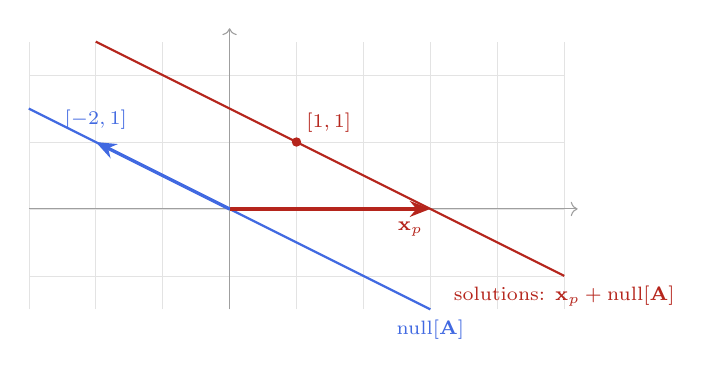
\begin{tikzpicture}[scale=0.85]
  \draw[step=1cm,gray!22,very thin] (-3,-1.5) grid (5,2.5);
  \draw[axisline] (-3,0) -- (5.2,0);
  \draw[axisline] (0,-1.5) -- (0,2.7);
  \draw[RoyalBlue,thick] (-3,1.5) -- (3,-1.5)
       node[below,font=\scriptsize]{$\nullsp{\mt{A}}$};
  \draw[BrickRed,thick] (-2,2.5) -- (5,-1)
       node[below,font=\scriptsize]{solutions: $\vc{x}_p+\nullsp{\mt{A}}$};
  \draw[vecarr,BrickRed] (0,0) -- (3,0);
  \node[below,font=\scriptsize,BrickRed] at (2.7,-0.05) {$\vc{x}_p$};
  \fill[BrickRed] (1,1) circle (2pt) node[above right,font=\scriptsize]{$[1,1]$};
  \draw[vecarr,RoyalBlue] (0,0) -- (-2,1);
  \node[above,font=\scriptsize,RoyalBlue] at (-2,1.05) {$[-2,1]$};
\end{tikzpicture}
\end{center}

%------------------------------------------------------------------------------
\subsection{The null space is orthogonal to the row space}
%------------------------------------------------------------------------------
By the row reading (\S2.3, \S11.3), $\mt{A}\vc{x}=\vc{0}$ says that every row of
$\mt{A}$ has dot product $0$ with $\vc{x}$. A vector orthogonal to each of the
rows is orthogonal to every combination of them, by linearity of the dot product
(the vector unit, \S21.1). So:

\begin{thm}
\label{thm:nullperp}
Every vector of $\nullsp{\mt{A}}$ is orthogonal to every vector of
$\rowsp{\mt{A}}$.
\end{thm}

\noindent In Example~\ref{ex:nulls}(e), $[\,-2,-3,1\,]$ is orthogonal to both rows:
$-2+0+2=0$ and $0-3+3=0$. The null space and the row space are two
perpendicular subspaces of the input space $\R^{n}$.

%==============================================================================
\section{The rank--nullity theorem}
%==============================================================================

%------------------------------------------------------------------------------
\subsection{A pattern}
%------------------------------------------------------------------------------
Collect the examples so far.
\begin{center}
\renewcommand{\arraystretch}{1.3}
\begin{tabular}{@{}l c c c@{}}
\toprule
\textbf{Matrix} & $n$ (columns) & rank & nullity \\
\midrule
$\mt{I}_2$ & $2$ & $2$ & $0$ \\
$2\times2$ zero matrix & $2$ & $0$ & $2$ \\
$\smat{1&2\\2&4}$ & $2$ & $1$ & $1$ \\
$\mt{P}_{\vc{u}}$ in $\R^{2}$ & $2$ & $1$ & $1$ \\
$\smat{1&0&2\\0&1&3}$ & $3$ & $2$ & $1$ \\
$\vc{u}\vc{v}\T$ in $\R^{3\times3}$ & $3$ & $1$ & $2$ \\
\bottomrule
\end{tabular}
\end{center}
In every row, rank plus nullity is the number of columns. The intuition is a
budget. The input space has $n$ dimensions. The matrix crushes some of them to
$\vc{0}$, the nullity, and the rest survive into the output as the column
space.

\begin{thm}[Rank--nullity]
\label{thm:ranknullity}
For every $\mt{A}\in\R^{m\times n}$,
\[
  \boxed{\;\rank(\mt{A})+\nullity(\mt{A})=n,\;}
\]
the number of columns of $\mt{A}$.
\end{thm}

%------------------------------------------------------------------------------
\subsection{What the proof uses}
%------------------------------------------------------------------------------
\lookback Three facts about dimension. The vector unit proved them in $\R^{2}$
and $\R^{3}$ and used them in $\R^{n}$ (\S17, \S24), and they are taken as given
here, as Part 1 \S1.1 took the fact that $n$ independent vectors span $\R^{n}$.
\begin{enumerate}[label=\textbf{F\arabic*.},leftmargin=2.6em,itemsep=2pt]
  \item Every subspace of $\R^{n}$ has a basis.
  \item Any linearly independent set of vectors in a subspace can be extended
        (by adding vectors) to a basis of that subspace.
  \item All bases of a subspace have the same number of vectors, its dimension.
\end{enumerate}

%------------------------------------------------------------------------------
\subsection{The proof}
%------------------------------------------------------------------------------
\begin{proof}[Proof of Theorem~\ref{thm:ranknullity}]
Let $p=\nullity(\mt{A})$ and let $\vc{k}_1,\dots,\vc{k}_p$ be a basis of
$\nullsp{\mt{A}}$ (F1). These are independent vectors of $\R^{n}$, so by F2 they
can be extended to a basis of $\R^{n}$,
\[
  \vc{k}_1,\dots,\vc{k}_p,\ \vc{w}_1,\dots,\vc{w}_r,
  \qquad p+r=n \text{ by F3}.
\]
The claim is that $\mt{A}\vc{w}_1,\dots,\mt{A}\vc{w}_r$ is a basis of
$\colsp{\mt{A}}$. Then $\rank(\mt{A})=r=n-p$, which is the theorem.

\emph{They span $\colsp{\mt{A}}$.} Any vector of the column space is
$\mt{A}\vc{x}$ for some $\vc{x}$. Write $\vc{x}$ in the basis,
$\vc{x}=c_1\vc{k}_1+\cdots+c_p\vc{k}_p+d_1\vc{w}_1+\cdots+d_r\vc{w}_r$. Since
$\mt{A}\vc{k}_i=\vc{0}$,
\[
  \mt{A}\vc{x}=d_1\mt{A}\vc{w}_1+\cdots+d_r\mt{A}\vc{w}_r .
\]

\emph{They are independent.} Suppose
$d_1\mt{A}\vc{w}_1+\cdots+d_r\mt{A}\vc{w}_r=\vc{0}$. Then
$\mt{A}(d_1\vc{w}_1+\cdots+d_r\vc{w}_r)=\vc{0}$, so
$d_1\vc{w}_1+\cdots+d_r\vc{w}_r$ is in the null space and is a combination of
the $\vc{k}$'s:
\[
  d_1\vc{w}_1+\cdots+d_r\vc{w}_r=c_1\vc{k}_1+\cdots+c_p\vc{k}_p .
\]
Moving everything to one side gives a combination of the basis vectors
$\vc{k}_1,\dots,\vc{k}_p,\vc{w}_1,\dots,\vc{w}_r$ equal to $\vc{0}$. A basis is
independent, so every coefficient is zero, in particular every $d_j$.
\end{proof}

\noindent The proof also says \emph{which} part of the input survives: the
directions $\vc{w}_j$ added to the null space are carried one-for-one onto a
basis of the column space.

%------------------------------------------------------------------------------
\subsection{Many examples}
%------------------------------------------------------------------------------
The theorem predicts nullities without solving anything, and it predicts ranks
from null spaces found by inspection.
\begin{ex}
\leavevmode
\begin{enumerate}[label=(\alph*),leftmargin=2em,itemsep=4pt]
  \item $\begin{bmatrix}1&0&1\\0&1&1\\1&1&2\end{bmatrix}$ has rank $2$ (\S12.3),
        so nullity $3-2=1$. The dependence $\vc{a}_1+\vc{a}_2-\vc{a}_3=\vc{0}$
        gives the null space: $\spanop\{[\,1,1,-1\,]\}$.
  \item $\begin{bmatrix}1&0\\0&1\\0&0\end{bmatrix}$: rank $2$, so nullity
        $2-2=0$. Independent columns, trivial null space.
  \item The $1\times n$ row $\begin{bmatrix}1&1&\cdots&1\end{bmatrix}$: rank $1$,
        so nullity $n-1$. Its null space is the set of vectors whose entries sum
        to $0$, a ``plane'' of dimension $n-1$ in $\R^{n}$.
  \item $\mt{R}_\theta$: rank $2$, nullity $0$. A rotation crushes nothing.
  \item $\mt{P}_{\vc{u}}$ in $\R^{n}$: rank $1$, so nullity $n-1$. The null
        space is everything perpendicular to $\vc{u}$.
  \item $\mt{I}-\mt{P}_{\vc{u}}$ in $\R^{n}$: it kills exactly the multiples
        of $\vc{u}$, so nullity $1$ and rank $n-1$.
  \item The $3\times3$ shear $\begin{bmatrix}1&k&0\\0&1&0\\0&0&1\end{bmatrix}$:
        independent columns, rank $3$, nullity $0$.
  \item $\vc{u}\vc{v}\T\in\R^{m\times n}$ with $\vc{u},\vc{v}\neq\vc{0}$: rank
        $1$, nullity $n-1$.
  \item \emph{Any} $4\times6$ matrix has rank at most $4$, so nullity at least
        $6-4=2$. Without seeing a single entry, we know $\mt{A}\vc{x}=\vc{0}$ has
        a plane's worth of solutions at least.
\end{enumerate}
\end{ex}

%------------------------------------------------------------------------------
\subsection{Consequences}
%------------------------------------------------------------------------------
\begin{cor}[Square matrices]
\label{cor:square}
For $\mt{A}\in\R^{n\times n}$ the following are equivalent: $\nullsp{\mt{A}}=\{\vc{0}\}$;
$\rank(\mt{A})=n$; $\colsp{\mt{A}}=\R^{n}$. In words, for a square matrix,
columns that are independent also span, and columns that span are also
independent.
\end{cor}

\begin{proof}
Rank--nullity gives the first equivalence. For the second, an $n$-dimensional
subspace of $\R^{n}$ is all of $\R^{n}$: by F2 its basis extends to a basis of
$\R^{n}$, but by F3 that basis already has $n$ vectors, so nothing is added.
\end{proof}

\noindent This is the fact Part 1 \S1.1 took on trust: $n$ independent vectors in
$\R^{n}$ form a basis. It follows from F1--F3 and rank--nullity. For a square
system $\mt{A}\vc{x}=\vc{b}$ it means: a unique solution for one $\vc{b}$, a
unique solution for every $\vc{b}$, and independent columns all stand or fall
together.

\begin{cor}[Wide and tall matrices]
\label{cor:widetall}
Let $\mt{A}\in\R^{m\times n}$.
\begin{itemize}[leftmargin=1.4em,itemsep=2pt]
  \item If $m<n$ (more unknowns than equations), $\nullity(\mt{A})\ge n-m>0$: the
        homogeneous system $\mt{A}\vc{x}=\vc{0}$ has nonzero solutions.
  \item If $m>n$ (more equations than unknowns), $\rank(\mt{A})\le n<m$, so
        $\colsp{\mt{A}}\neq\R^{m}$: some right-hand sides $\vc{b}$ have no
        solution.
\end{itemize}
\end{cor}

%==============================================================================
\section{A corollary: \texorpdfstring{$\rank(\mt{A}\T\mt{A})=\rank(\mt{A})$}{rank(A'A) = rank(A)}}
%==============================================================================

%------------------------------------------------------------------------------
\subsection{The same null space}
%------------------------------------------------------------------------------
For any $\mt{A}\in\R^{m\times n}$, the product $\mt{A}\T\mt{A}$ is square,
$n\times n$, and symmetric (\S8.6, P4). It turns up wherever lengths are squared,
as in \S20 and Part 9. Its null space is the null space of $\mt{A}$.

\begin{thm}
\label{thm:samenull}
$\nullsp{\mt{A}\T\mt{A}}=\nullsp{\mt{A}}$.
\end{thm}

\begin{proof}
If $\mt{A}\vc{x}=\vc{0}$, then $\mt{A}\T\mt{A}\vc{x}=\mt{A}\T\vc{0}=\vc{0}$. So
$\nullsp{\mt{A}}\subseteq\nullsp{\mt{A}\T\mt{A}}$.

Conversely, suppose $\mt{A}\T\mt{A}\vc{x}=\vc{0}$. Multiply on the left by
$\vc{x}\T$:
\[
  0=\vc{x}\T\mt{A}\T\mt{A}\vc{x}=(\mt{A}\vc{x})\T(\mt{A}\vc{x})=\norm{\mt{A}\vc{x}}^{2},
\]
using M6 and \S7.3. A vector of length zero is the zero vector, so
$\mt{A}\vc{x}=\vc{0}$.
\end{proof}

%------------------------------------------------------------------------------
\subsection{The same rank}
%------------------------------------------------------------------------------
\begin{cor}
\label{cor:ATA}
For every $\mt{A}\in\R^{m\times n}$, $\rank(\mt{A}\T\mt{A})=\rank(\mt{A})$.
\end{cor}

\begin{proof}
$\mt{A}$ and $\mt{A}\T\mt{A}$ both have $n$ columns, and by
Theorem~\ref{thm:samenull} the same nullity. By rank--nullity,
$\rank(\mt{A}\T\mt{A})=n-\nullity(\mt{A}\T\mt{A})=n-\nullity(\mt{A})=\rank(\mt{A})$.
\end{proof}

\begin{ex}
$\mt{A}=\begin{bmatrix}1&2\\2&4\\3&6\end{bmatrix}$ has rank $1$ (the second column
is twice the first), and
$\mt{A}\T\mt{A}=\begin{bmatrix}14&28\\28&56\end{bmatrix}$ has rank $1$ too.
$\mt{B}=\begin{bmatrix}1&0\\0&1\\1&1\end{bmatrix}$ has rank $2$, and
$\mt{B}\T\mt{B}=\begin{bmatrix}2&1\\1&2\end{bmatrix}$ has determinant $3\neq0$,
so rank $2$.
\end{ex}

%------------------------------------------------------------------------------
\subsection{Row rank equals column rank}
%------------------------------------------------------------------------------
\S12.4 stated that $\dim\rowsp{\mt{A}}=\dim\colsp{\mt{A}}$ for every matrix and
checked it for $2\times2$. Here is the proof.

\begin{cor}
\label{cor:rowrank}
For every $\mt{A}\in\R^{m\times n}$, $\rank(\mt{A}\T)=\rank(\mt{A})$. That is,
$\dim\rowsp{\mt{A}}=\dim\colsp{\mt{A}}$.
\end{cor}

\begin{proof}
Every column of $\mt{A}\T\mt{A}$ is $\mt{A}\T$ times a column of $\mt{A}$, hence
a combination of the columns of $\mt{A}\T$. So
$\colsp{\mt{A}\T\mt{A}}\subseteq\colsp{\mt{A}\T}$, and a subspace inside another
has no larger dimension (extend its basis by F2). Hence, with
Corollary~\ref{cor:ATA},
\[
  \rank(\mt{A})=\rank(\mt{A}\T\mt{A})\le\rank(\mt{A}\T).
\]
This holds for \emph{every} matrix, so it holds for $\mt{A}\T$ in place of
$\mt{A}$: $\rank(\mt{A}\T)\le\rank\bigl((\mt{A}\T)\T\bigr)=\rank(\mt{A})$. The two
inequalities together give equality. Finally $\rank(\mt{A}\T)=\dim\colsp{\mt{A}\T}
=\dim\rowsp{\mt{A}}$ (\S11.1).
\end{proof}

%------------------------------------------------------------------------------
\subsection{When \texorpdfstring{$\mt{A}\T\mt{A}$}{A'A} has full rank}
%------------------------------------------------------------------------------
\begin{cor}
\label{cor:ATAfull}
$\mt{A}\T\mt{A}$ has full rank $n$ if and only if $\mt{A}$ has full column rank,
i.e.\ the columns of $\mt{A}$ are independent.
\end{cor}

\noindent This is the hinge of least squares in Part 9: the system that
produces the best approximate solution has the matrix $\mt{A}\T\mt{A}$, and this
corollary says when it has exactly one solution.

%==============================================================================
\section{The \texorpdfstring{$2\times2$}{2x2} inverse}
%==============================================================================

%------------------------------------------------------------------------------
\subsection{Undoing a matrix}
%------------------------------------------------------------------------------
The scalar equation $ax=b$ is solved by $x=a^{-1}b$ when $a\neq0$, because
$a^{-1}a=1$. Part 1 \S2.4 noted the resemblance between $ax=b$ and
$\mt{A}\vc{x}=\vc{b}$ and warned that there was as yet no meaning for
$\mt{A}^{-1}$. If there were a matrix $\mt{B}$ with $\mt{B}\mt{A}=\mt{I}$, then
multiplying $\mt{A}\vc{x}=\vc{b}$ by $\mt{B}$ would give
$\vc{x}=\mt{B}\mt{A}\vc{x}=\mt{B}\vc{b}$.

\begin{defn}[Inverse of a $2\times2$ matrix]
$\mt{A}\in\R^{2\times2}$ is \textbf{invertible} if there is a matrix $\mt{B}$
with $\mt{A}\mt{B}=\mt{B}\mt{A}=\mt{I}$. Then $\mt{B}$ is the \textbf{inverse}
of $\mt{A}$, written $\mt{A}^{-1}$.
\end{defn}

\noindent There is at most one. If $\mt{B}\mt{A}=\mt{I}$ and $\mt{A}\mt{C}=\mt{I}$,
then by associativity
$\mt{B}=\mt{B}(\mt{A}\mt{C})=(\mt{B}\mt{A})\mt{C}=\mt{C}$.

%------------------------------------------------------------------------------
\subsection{Finding it}
%------------------------------------------------------------------------------
Write $\mt{A}=\begin{bmatrix}a&b\\c&d\end{bmatrix}$ and look for $\mt{X}$ with
$\mt{A}\mt{X}=\mt{I}$. Column by column (the column reading of a product), this
is two systems: $\mt{A}\vc{x}_1=\vc{e}_1$ and $\mt{A}\vc{x}_2=\vc{e}_2$. The
first is
\[
  ax+by=1,\qquad cx+dy=0 .
\]
Multiply the first equation by $d$, the second by $b$, and subtract:
$(ad-bc)\,x=d$. Multiply the first by $c$, the second by $a$, and subtract:
$(bc-ad)\,y=c$. So if $ad-bc\neq0$,
\[
  \vc{x}_1=\frac{1}{ad-bc}\begin{bmatrix}d\\-c\end{bmatrix},
  \qquad\text{and in the same way}\qquad
  \vc{x}_2=\frac{1}{ad-bc}\begin{bmatrix}-b\\a\end{bmatrix}.
\]
The denominator is $\det\mt{A}$.

\begin{thm}[The $2\times2$ inverse]
\label{thm:inv2}
If $\det\mt{A}=ad-bc\neq0$, then
\[
  \boxed{\;\mt{A}^{-1}=\frac{1}{ad-bc}\begin{bmatrix}d&-b\\-c&a\end{bmatrix}.\;}
\]
\end{thm}

\begin{proof}
Multiply in both orders:
\[
  \begin{bmatrix}a&b\\c&d\end{bmatrix}\begin{bmatrix}d&-b\\-c&a\end{bmatrix}
  =\begin{bmatrix}ad-bc&0\\0&ad-bc\end{bmatrix},
  \qquad
  \begin{bmatrix}d&-b\\-c&a\end{bmatrix}\begin{bmatrix}a&b\\c&d\end{bmatrix}
  =\begin{bmatrix}ad-bc&0\\0&ad-bc\end{bmatrix},
\]
and divide by $ad-bc$.
\end{proof}

\noindent The recipe: \emph{swap the diagonal entries, negate the off-diagonal
entries, divide by the determinant.}

%------------------------------------------------------------------------------
\subsection{When there is no inverse}
%------------------------------------------------------------------------------
\begin{thm}
\label{thm:inv2iff}
For $\mt{A}\in\R^{2\times2}$ the following are equivalent:
$\mt{A}$ is invertible; $\det\mt{A}\neq0$; $\rank\mt{A}=2$;
$\nullsp{\mt{A}}=\{\vc{0}\}$.
\end{thm}

\begin{proof}
If $\det\mt{A}\neq0$, Theorem~\ref{thm:inv2} produces the inverse. If $\mt{A}$
is invertible and $\mt{A}\vc{x}=\vc{0}$, then
$\vc{x}=\mt{A}^{-1}\mt{A}\vc{x}=\vc{0}$, so the null space is $\{\vc{0}\}$. That
gives rank $2$ by rank--nullity, and rank $2$ gives $\det\mt{A}\neq0$ by \S14.2.
\end{proof}

\noindent The geometry is the null space of \S31.5. A matrix with
$\det\mt{A}=0$ merges different inputs into one output. No matrix $\mt{B}$ could
send that one output back to two different places, so nothing can undo
$\mt{A}$. A projection, which forgets a whole line, is the typical example.

\noindent One more property follows from P8 of \S22: if $\mt{A}$ is invertible,
$\det\mt{A}\,\det\mt{A}^{-1}=\det\mt{I}=1$, so
$\det\mt{A}^{-1}=1/\det\mt{A}$. Undoing a matrix undoes its area factor.

%------------------------------------------------------------------------------
\subsection{The gallery, inverted}
%------------------------------------------------------------------------------
\begin{ex}
\leavevmode
\begin{itemize}[leftmargin=1.4em,itemsep=4pt]
  \item \textbf{Rotation.} $\det\mt{R}_\theta=1$, and the recipe gives
        $\mt{R}_\theta^{-1}=\begin{bmatrix}\cos\theta&\sin\theta\\-\sin\theta&\cos\theta\end{bmatrix}
        =\mt{R}_{-\theta}=\mt{R}_\theta\T$: rotate back (\S24.6).
  \item \textbf{Shear.} $\begin{bmatrix}1&k\\0&1\end{bmatrix}^{-1}=\begin{bmatrix}1&-k\\0&1\end{bmatrix}$:
        slide back.
  \item \textbf{Scaling.} $\diagop(s_1,s_2)^{-1}=\diagop(1/s_1,1/s_2)$, when
        $s_1s_2\neq0$.
  \item \textbf{Reflection.} A reflection undoes itself: $\mt{F}^{-1}=\mt{F}$.
  \item \textbf{Orthogonal.} For any $2\times2$ orthogonal $\mt{Q}$,
        $\mt{Q}\T\mt{Q}=\mt{Q}\mt{Q}\T=\mt{I}$ says exactly $\mt{Q}^{-1}=\mt{Q}\T$.
  \item \textbf{Projection.} $\det\mt{P}_{\vc{u}}=0$: no inverse.
\end{itemize}
\end{ex}

%------------------------------------------------------------------------------
\subsection{Solving with it}
%------------------------------------------------------------------------------
Part 1 \S1.5 solved
$\begin{bmatrix}2&1\\1&3\end{bmatrix}\vc{x}=\begin{bmatrix}5\\5\end{bmatrix}$ by
substitution and got $\vc{x}=[\,2,1\,]$. Now $\det=6-1=5$ and
\[
  \vc{x}=\mt{V}^{-1}\vc{u}
  =\frac15\begin{bmatrix}3&-1\\-1&2\end{bmatrix}\begin{bmatrix}5\\5\end{bmatrix}
  =\frac15\begin{bmatrix}10\\5\end{bmatrix}
  =\begin{bmatrix}2\\1\end{bmatrix}. \quad\checkmark
\]
This is the matrix meaning of $x=b/a$ promised in Part 1 \S2.4.

Inverses of products reverse the order, like transposes (M6): if $\mt{A}$ and
$\mt{B}$ are invertible then
$(\mt{A}\mt{B})(\mt{B}^{-1}\mt{A}^{-1})=\mt{A}(\mt{B}\mt{B}^{-1})\mt{A}^{-1}=\mt{A}\mt{A}^{-1}=\mt{I}$,
so $(\mt{A}\mt{B})^{-1}=\mt{B}^{-1}\mt{A}^{-1}$. To undo ``$\mt{B}$, then
$\mt{A}$'', undo $\mt{A}$ first.

%------------------------------------------------------------------------------
\subsection{Practice}
%------------------------------------------------------------------------------
\begin{enumerate}[label=\textbf{P\arabic*.},leftmargin=2.6em,itemsep=5pt]
  \item Find the null space and nullity of
        $\begin{bmatrix}1&-1&2\\2&-2&4\end{bmatrix}$, and check rank--nullity.
  \item Without computing, give the smallest possible nullity of a $5\times8$
        matrix and the largest possible rank of a $7\times3$ matrix.
  \item Find all solutions of $x_1+2x_2-x_3=4$ (one equation, three unknowns) in
        the form $\vc{x}_p+\nullsp{\mt{A}}$.
  \item Which lines through the origin are invariant under
        $\diagop(2,3)$? Under $3\mt{I}$?
  \item For $\mt{A}=\begin{bmatrix}1&1\\1&1\\0&0\end{bmatrix}$, compute
        $\mt{A}\T\mt{A}$ and check that the ranks agree.
  \item Invert $\begin{bmatrix}4&7\\2&6\end{bmatrix}$ and use the inverse to solve
        $\begin{bmatrix}4&7\\2&6\end{bmatrix}\vc{x}=\begin{bmatrix}1\\2\end{bmatrix}$.
\end{enumerate}

\subsubsection*{Answers}

\noindent\textbf{P1.} Both rows say $x_1-x_2+2x_3=0$. With $x_2=s$ and $x_3=t$
free, $x_1=s-2t$, so
$\nullsp{\mt{A}}=\spanop\{[\,1,1,0\,],[\,-2,0,1\,]\}$, nullity $2$. The rank is
$1$, and $1+2=3$. \checkmark

\smallskip
\noindent\textbf{P2.} Rank at most $5$, so nullity at least $8-5=3$. Rank at most
$\min(7,3)=3$.

\smallskip
\noindent\textbf{P3.} $\vc{x}_p=[\,4,0,0\,]$; the null space of
$\begin{bmatrix}1&2&-1\end{bmatrix}$ is $\spanop\{[\,-2,1,0\,],[\,1,0,1\,]\}$; so
$\vc{x}=[\,4,0,0\,]+s[\,-2,1,0\,]+t[\,1,0,1\,]$, a plane in $\R^{3}$ not through
the origin.

\smallskip
\noindent\textbf{P4.} $\diagop(2,3)$: only the two axes. If $[\,x,y\,]\mapsto[\,2x,3y\,]$
is a multiple $\lambda[\,x,y\,]$ with $x,y$ both nonzero, then $\lambda=2=3$,
impossible. $3\mt{I}$: every line, since every vector is only stretched.

\smallskip
\noindent\textbf{P5.} $\mt{A}\T\mt{A}=\begin{bmatrix}2&2\\2&2\end{bmatrix}$, rank $1$;
$\mt{A}$ has two equal columns, rank $1$. \checkmark

\smallskip
\noindent\textbf{P6.} $\det=24-14=10$, so
$\mt{A}^{-1}=\frac{1}{10}\begin{bmatrix}6&-7\\-2&4\end{bmatrix}$ and
$\vc{x}=\frac{1}{10}[\,6-14,\ -2+8\,]=[\,-0.8,\ 0.6\,]$. Check:
$4(-0.8)+7(0.6)=1$ and $2(-0.8)+6(0.6)=2$. \checkmark

\lookahead The $2\times2$ determinant has done a great deal: it measures area,
detects rank, and builds the inverse. Part 7 defines the determinant of an
$n\times n$ matrix, by expanding along a row, and proves the properties that
make it as useful in every dimension as it has been in the plane.

\end{document}
